
\section{Torsionspendel}
In dem zweiten Versuch wurde mit einem Torsionspendel der Schubmodul sowie das Rückstelldrehmoment des Drahtes berechnet.
Im Abgleich mit Literaturwerten wird dann die Behauptung gestützt, dass der Draht aus Stahl besteht, da sein errechneter Schubmodul nahe am Literaturwert des Schubmoduls von Stahl liegt.
Zur Messung werden eine rotierende Scheibe, sowie eine Hantel mit verstellbaren Gewichten genutzt.
Von diesen soll zusätzlich das Trägheitsmoment bestimmt werden.

\subsection{Methoden}
Das Torsionspendel bestand aus einem dünnen Draht, welches fest an einer Halterung angebracht war.
Am unteren Ende des Drahtes konnten durch einen Schraubmechanismus eine flach zylindrische Metallscheibe und eine Hantel mit abnehmbaren- und auf der Achse verschiebbaren Gewichtsscheiben angebracht werden.
Dabei dienten Kerben in der Achse dazu, die Gewichte in festen Abständen vom Mittelpunkt aus zu fixieren.
Zudem konnten die Gewichte komplett von der Hantelachse entfernt werden.
Es wurden nun die Zeiten über jeweils mehrere Schwingungsperioden gemessen.

Für die analoge Zeitmessung wird eine Unsicherheit von $u(T) = \frac{\SI{0,1}{\second}}{2\sqrt{6}}\approx \SI{20}{\milli\second}$ angenommen.
Da die Scheibe eine kleine Markierung hatte, konnte die Zeit gut anhand der Ruhelage abgeschätzt werden.
Dabei wurde die Auslenkung in Ruhelage durch einen Stab hinter der Scheibe bzw. der Hantel markiert.

Der Draht hatte eine Länge von \SI{181}{\centi\meter}.
Da das Maßband sich ein wenig gebogen hat, kann hier eine Unsicherheit von $u(L) = \frac{\SI{5}{\milli\meter}}{2\sqrt6}\approx \SI{1,0}{\milli\meter}$ angenommen werden.
Für weitere Längenmessungen mit dem Maßband kann der Wert besser abgelesen werden und es sei $u(R_z) = \frac{\SI{1}{\milli\meter}}{2\sqrt{6}} \approx \SI{0,20}{\milli\meter}$.

Um sicher zu gehen, dass der Draht überall die gleiche Dicke aufweist, wurde dieser an fünf verschiedenen Stellen jeweils drei mal gemessen.
Der erste gemessene Wert war hierbei stets größer als die nachfolgenden, was auf eine Deformation des Drahtes beim messen hindeutet.
Aufgrund dieser erheblichen Deformation von bis zu $20\%$ wird im folgenden nur der erste Wert jeder Messung betrachtet.
Alle Werte der jeweils ersten Messung liegen nah beieinander und der Draht kann als gleichmäßig dick angesehen werden mit $R = \SI{0,25 +- 0,05}{\milli\meter}$.

\subsection{Datenauswertung}

\subsubsection*{Rotationsscheibe}
Es wurden neun Schwingungsperioden gemessen.
Damit ergibt sich eine Schwingungsdauer von \SI{33,00 +- 0,00}{\second}\footnote{Genauere Werte finden sich im Anhang in Tab. \ref{tab:schwingungsperioden}}.
Die Scheibe hat einen Durchmesser von \SI{15}{\centi\meter} und ein Gewicht von \SI{2,648}{\kilogram}.
Nach Gl. (34)\footnote{Hier ist die Gl. (34) in der Einführung gemeint und noch einmal angegeben.}
\begin{equation}
	G = \frac{4\pi L m_z R_z^2}{R^4 T^2}
\end{equation}
ist der Schubmodul gegeben mit $G = \SI{79,66+-13,02}{\giga\pascal}$\footnote{Für Unsicherheitsrechnungen siehe Anhang Gl. (\ref{eq:G-unc})}.

\subsubsection*{Hantel}
Es wurden für jede Konfiguration drei Schwingungsperioden gemessen.
Trägt man wie in Abb. \ref{fig:hantel-fit} dargestellt $T^2$ gegen $2 \, m_2 \, a^2$ auf, so kann man einen linearen Zusammenhang erkennen.
Hierbei wurde die Konfiguration ohne Hantelscheiben noch nicht betrachtet.
\begin{figure}[ht]
	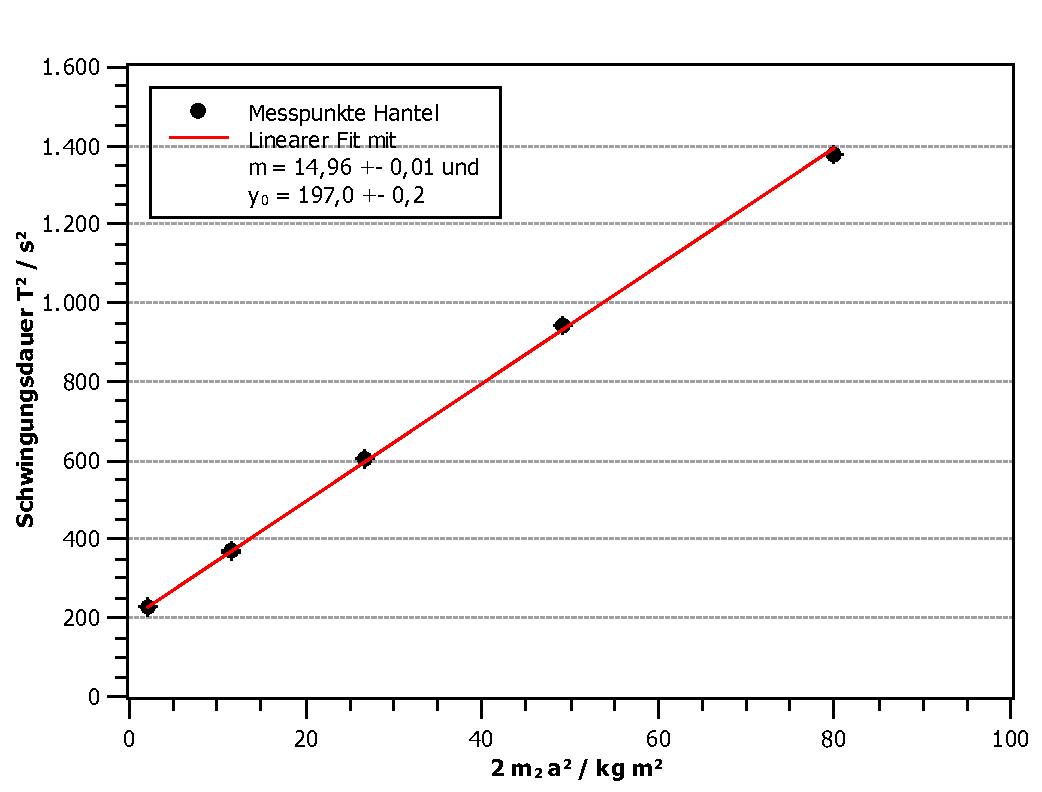
\includegraphics[width=\textwidth]{Torsion_Hantel_linear.pdf}
	\caption{Ausgleichsgerade durch linearisierte Messwerte. (Unsicherheiten kleiner als Symbole.)}
	\label{fig:hantel-fit}
\end{figure}
Durch einen linearen Fit\footnote{Programm: SciDaVis; Algorithmus: kleinste Quadrate} kann die Steigung $m$ ermittelt und nach Gl. (43) 
\begin{equation}
	\label{eq:hantel-t2}
	T^2 = \frac{4\pi^2}{D^*} (J_1 + 2 J_2 + 2 m_2 a^2)
\end{equation}
folgt $m = \frac{4\pi}{D^*}$.
(Es sei zu bedenken, dass $m$ von der Einheit \si{\second\squared\per\kilogram\per\meter\squared} $=$ \si{\per\newton\per\meter} ist.)
Daraus folgt ein rücktreibendes Direktionsmoment von 
\begin{equation}
	D^* = \frac{4\pi}{m} \approx \SI{2,640+-0,002}{\newton\meter}.
\end{equation}

Das Trägheitsmoment $J_1$ der Hantelachse kann im Spezialfall $m_2 = 0$ sowie $J_2 = 0$, d. h. ohne Gewichte, mit Gl. (\ref{eq:hantel-t2}) bestimmt werden.
Es folgt $J_1 = \frac{T^2 D^*}{4\pi^2} \approx \SI{11,74 +- 0,02}{\kilogram\meter\squared}$.

Formt man Gl. (\ref{eq:hantel-t2}) nach $J_2$ um, so ist für $a = 0$ und $T^2 = y_0$ aus Abb. \ref{fig:hantel-fit} das Trägheitsmoment einer Hantelscheibe gegeben mit
\begin{equation}
	J_2 = \frac{\frac{y_0 D^*}{4 \pi^2} - J_1}{2} \approx \SI{0,7176 +- 0,0121}{\kilogram\meter\squared}.
\end{equation}

\subsection{Schlussfolgerung}
Durch die Messung eines Torsionspendels, konnte der Schubmodul für das Material des Drahtes auf $G = \SI{79,66+-13,02}{\giga\pascal}$ ermittelt werden.
Das Ergebnis scheint dem Literaturwert von Stahl mit \SI{79,3}{\giga\pascal}\footnote{Wert nach Wikipedia aus Crandall, Dahl, Lardner: An Introduction to the Mechanics of Solids. McGraw-Hill, 1959} sehr nahe zu kommen, es wurden bei dem Versuch jedoch teilweise große Abschätzungen gemacht, was an der hohen relativen Unsicherheit von ca. $16\%$ erkennbar ist.
Dennoch kann die Hypothese eines Stahldrahtes unterstützt werden, da z. B. Aluminium ein Schubmodul von $\SI{25,5}{\giga\pascal}$ besitzt und somit außerhalb eines akzeptablen Vertrauensgrades liegt.

Um den Literaturwert genau zu überprüfen, muss die Dicke des Draht deutlich genauer gemessen werden.
Da der Schubmodul mit der vierten Potenz von dem Radius des Drahtes abhängt, muss eine Methode gefunden werden, welche die Mikrometerschraube stets mit der gleichen Kraft anzieht.
Zusätzlich sollte diese Kraft möglichst gering gehalten werden, um den Draht nicht beim messen zu deformieren.

Für das rücktreibende Drehmoment des Drahtes ist ein Wert von \SI{2,640+-0,002}{\newton\meter} bestimmt worden.
Das Trägheitsmoment für die Hantelachse ist auf einen Wert von \SI{11,74 +- 0,02}{\kilogram\meter\squared} bestimmt worden, während das der Hantelgewichte nur \SI{0,7176 +- 0,0121}{\kilogram\meter\squared} betrug.
Diese große Differenz vermögen wir nicht zu erklären und es ist ratsam, auch diese Messung ggf. mit mehr Schwingungsperioden zu wiederholen.
